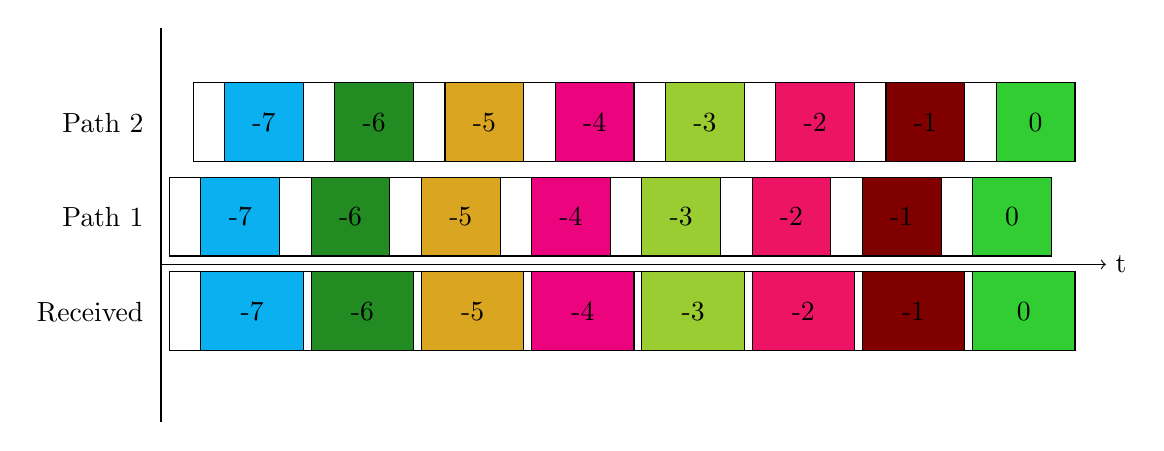
\begin{tikzpicture}
  \tikzset{
    sample/.style={minimum width=10mm, minimum height=10mm, anchor=south west, draw=black},
    rcp/.style={minimum width=4mm, minimum height=10mm, anchor=south west, draw=black, fill=white},
    rnarrow/.style={minimum width=1mm, minimum height=10mm, anchor=south west, draw=black, fill=white},
    wsample/.style={minimum width=13mm, minimum height=10mm, anchor=south west, draw=black},
    label/.style={anchor=east},
  }

  % time axis
  \draw[->]
  (0, 0) --
  (12, 0) node[anchor=west]{t};

  % other axis
  \draw
  (0, -2) --
  (0, 3);

  % Path 1
  \draw
  (0.1, 0.1) node[rcp]{}
  ++(0.4, 0) node[sample, fill=ProcessBlue]{-7}
  ++(1, 0)node[rcp]{}
  ++(0.4, 0) node[sample, fill=ForestGreen]{-6}
  ++(1, 0)node[rcp]{}
  ++(0.4, 0) node[sample, fill=Goldenrod]{-5}
  ++(1, 0)node[rcp]{}
  ++(0.4, 0) node[sample, fill=RubineRed]{-4}
  ++(1, 0)node[rcp]{}
  ++(0.4, 0) node[sample, fill=YellowGreen]{-3}
  ++(1, 0)node[rcp]{}
  ++(0.4, 0) node[sample, fill=WildStrawberry]{-2}
  ++(1, 0)node[rcp]{}
  ++(0.4, 0) node[sample, fill=Maroon]{-1}
  ++(1, 0)node[rcp]{}
  ++(0.4, 0) node[sample, fill=LimeGreen]{0};

  % Path 2
  \draw
  (0.4, 1.3) node[rcp]{}
  ++(0.4, 0) node[sample, fill=ProcessBlue]{-7}
  ++(1, 0)node[rcp]{}
  ++(0.4, 0) node[sample, fill=ForestGreen]{-6}
  ++(1, 0)node[rcp]{}
  ++(0.4, 0) node[sample, fill=Goldenrod]{-5}
  ++(1, 0)node[rcp]{}
  ++(0.4, 0) node[sample, fill=RubineRed]{-4}
  ++(1, 0)node[rcp]{}
  ++(0.4, 0) node[sample, fill=YellowGreen]{-3}
  ++(1, 0)node[rcp]{}
  ++(0.4, 0) node[sample, fill=WildStrawberry]{-2}
  ++(1, 0)node[rcp]{}
  ++(0.4, 0) node[sample, fill=Maroon]{-1}
  ++(1, 0)node[rcp]{}
  ++(0.4, 0) node[sample, fill=LimeGreen]{0};

  % Received
  \draw
  (0.1, -1.1) node[rcp]{}
  ++(0.4, 0) node[wsample, fill=ProcessBlue]{-7}
  ++(1.3, 0)node[rnarrow]{}
  ++(0.1, 0) node[wsample, fill=ForestGreen]{-6}
  ++(1.3, 0)node[rnarrow]{}
  ++(0.1, 0) node[wsample, fill=Goldenrod]{-5}
  ++(1.3, 0)node[rnarrow]{}
  ++(0.1, 0) node[wsample, fill=RubineRed]{-4}
  ++(1.3, 0)node[rnarrow]{}
  ++(0.1, 0) node[wsample, fill=YellowGreen]{-3}
  ++(1.3, 0)node[rnarrow]{}
  ++(0.1, 0) node[wsample, fill=WildStrawberry]{-2}
  ++(1.3, 0)node[rnarrow]{}
  ++(0.1, 0) node[wsample, fill=Maroon]{-1}
  ++(1.3, 0)node[rnarrow]{}
  ++(0.1, 0) node[wsample, fill=LimeGreen]{0};

  \draw
  (-0.1, 0.6) node[label]{Path 1}
  (-0.1, 1.8) node[label]{Path 2}
  (-0.1, -0.6) node[label]{Received};
\end{tikzpicture}
